\documentclass{beamer}

\mode<presentation>
{
	\usetheme{Warsaw}
	\usepackage{graphicx}
	% or ...	
	
	\setbeamercovered{transparent,invisible}
	\setbeamertemplate{navigation symbols}{}
	% or whatever (possibly just delete it)
}

\usepackage[english]{babel}
% or whatever
\usepackage{graphicx,subfigure}
\usepackage[utf8]{inputenc}
% or whatever

\usepackage{times}
\usepackage[T1]{fontenc}
% Or whatever. Note that the encoding and the font should match. If T1
% does not look nice, try deleting the line with the fontenc.
\usepackage{amsthm}
\newtheorem*{mylim*}{Limitations}
\usepackage{gensymb}
\usepackage{hyperref}
\hypersetup{
	colorlinks=true,
	linkcolor=blue,
	anchorcolor=blue,
	filecolor=blue,      
	citecolor=blue,
	urlcolor=blue
}
\usepackage{url,graphicx,subfigure}
\usepackage{listings}
\usepackage{color}
\usepackage{soul}
\usepackage{xspace}
\usepackage{pifont}
\usepackage{cite}
\usepackage{lipsum}% http://ctan.org/pkg/lipsum
\usepackage{algpseudocode}% http://ctan.org/pkg/algorithmicx
\usepackage{graphicx}
\usepackage[compatibility=false]{caption}% http://ctan.org/pkg/caption
\usepackage{booktabs}
\usepackage{url}
\usepackage{multirow}
\usepackage{pgfplots}
\usepackage{tikz}
\usetikzlibrary{matrix,fit,shapes,calc,positioning,shadows,arrows,shapes,backgrounds,decorations.markings,fadings}
\usepgfplotslibrary{statistics}
\usepackage[normalem]{ulem}
\useunder{\uline}{\ul}{}
\usepackage[skins]{tcolorbox}
\usepackage[linesnumbered,lined,boxed,ruled,vlined]{algorithm2e}
\usepackage[labelformat=empty]{caption}
\usepackage{color, colortbl}
\definecolor{Gray}{gray}{0.9}
\usepackage{amsmath,amssymb,amsfonts}

\hyphenation{op-tical net-works semi-conduc-tor}

\definecolor{comments}{rgb}{0.25,0.5,0.35}

\definecolor{brass}{rgb}{0.71, 0.65, 0.26}

\definecolor{SM}{rgb}{0.5,0,1}
\newcommand {\rsm} {\color{SM}}

\newcommand{\disp}{\insertframenumber/\inserttotalframenumber}

\newcommand{\backupbegin}{
	\newcounter{finalframe}
	\setcounter{finalframe}{\value{framenumber}}
}
\newcommand{\backupend}{
	\setcounter{framenumber}{\value{finalframe}}
}

\definecolor{antiquefuchsia}{rgb}{0.7, 0.1, 0.85}
\definecolor{airforceblue}{rgb}{0.36, 0.54, 0.66}
\definecolor{brass}{rgb}{0.71, 0.65, 0.26}
\definecolor{indiagreen}{rgb}{0.07, 0.53, 0.03}
\definecolor{darkorange}{rgb}{1.0, 0.55, 0.0}
\definecolor{navyblue}{rgb}{0.36, 0.54, 0.66}
\definecolor{darkred}{rgb}{0.55, 0.0, 0.0}

\newcommand{\REM}[1]{}
\newcommand{\todo}[1]{\textrm{\color{blue} #1}}
\newcommand{\sm}[1]{\textrm{\color{red} #1}}
\newcommand{\colosseum}{\textsf{Colosseum}\xspace}
\newcommand{\hansie}{\textsf{Hansie}\xspace}
\newcommand{\mahtab}{\textsf{Mahtab}\xspace}
\newcommand{\overallspeedup}{\todo{XXX}}

\resetcounteronoverlays{algocf}

\newcommand{\smr}[1]{\textrm{\color{black} #1}}
\newcommand{\sms}[1]{\textrm{\color{black} #1}}
\renewcommand{\ttdefault}{pcr}
\lstset{
	language=Java,
	escapechar=|,
	numbers=left,
	stepnumber=1,
	numbersep=5pt,
	numberstyle=\tiny\color{gray},
	backgroundcolor=\color{white},
	stringstyle=\fontsize{7.5}{7.5}\selectfont\ttfamily,
	keywordstyle=\ttfamily,
	showspaces=false,
	showstringspaces=false,
	showtabs=false,
	tabsize=2,
	captionpos=b,
	breaklines=true,
	breakatwhitespace=true,
	title=\lstname,
	basicstyle=\fontsize{7.5}{7.5}\selectfont\ttfamily,
	commentstyle=\color{red},
}
\newcommand{\ie}{i.e.}
\newcommand{\eg}{e.g.}
\newcommand{\aka}{a.k.a.}
\newcommand{\etal}{et al.}  % and colleagues
\newcommand{\CodeIn}[1]{{\small{\texttt{#1}}}}
\newcommand{\CodeInTab}[1]{{\scriptsize{\texttt{#1}}}}
\newcommand{\FancyIn}[1]{{\small{\textsc{#1}}}}
\newcommand{\MyComment}[1]{}
% common names
\newcommand{\reveng}{Reverse Engineering}

%% review original
\newcommand{\Fix}[1]{{\textbf{[[}\color{magenta}#1}\textbf{]]}}
\newcommand{\Mar}[1]{{\textbf{[[Marcelo:~}\color{red}#1}\textbf{]]}}
\newcommand{\SM}[1]{{\textbf{[[Shouvick:~}\color{blue}#1}\textbf{]]}}
\newcommand{\Den}[1]{[\textbf{Denini}:~{\color{brown} #1}]}

% \newcommand{\Fix}[1]{}
% \newcommand{\Mar}[1]{}
% \newcommand{\SM}[1]{}
% \newcommand{\Den}[1]{}

%% numbers
\newcommand{\configClasses}{\CodeIn{classes}}
\newcommand{\configMethods}{\CodeIn{methods}}
\newcommand{\configClassesAndMethods}{\CodeIn{classesMethods}}
\newcommand{\configClassesTab}{\CodeInTab{classes}}
\newcommand{\configMethodsTab}{\CodeInTab{methods}}
\newcommand{\configClassesAndMethodsTab}{\CodeInTab{classesMethods}}

\newcommand{\tname}{\textsc{PASTE}}

\def\denseitems{
   \itemsep1pt plus1pt minus1pt
   \parsep0pt plus0pt
   \parskip0pt\topsep0pt}

%% numbers and names
\newcommand{\OurURL}{\url{https://github.com/STAR-RG/paste}}
\newcommand{\NumProjects}{25}
\newcommand{\NumProjectsSpeedups}{13}
\newcommand{\FrequencySpeedups}{52} % NumProjectsSpeedups/NumProjects (13/25)
\newcommand{\SpeedupClassesAvg}{1.47}
\newcommand{\SpeedupClassesMedian}{1.59}
\newcommand{\SpeedupClassesMax}{2.28}
\newcommand{\SpeedupClassesMin}{0.93}
\newcommand{\NumRepeatsExperiment}{5}
\newcommand{\NumRepeatsManifest}{10}
\newcommand{\NumProjectsParExecFails}{11}
\newcommand{\NumProjectsParExecFailsPercentage}{44}
\newcommand{\NumStars}{200}
\newcommand{\NumTests}{300}
\newcommand{\NumFailsAtlasStageOneMethods}{147.2}
\newcommand{\NumFailsAtlasStageOneMethodsNoFraction}{141.2}
\newcommand{\NumFailsAtlasStageTwoMethods}{6}
\newcommand{\NumFailsClassesTotalStageOne}{402.6}
\newcommand{\NumFailsClassesAndMethodsTotalStageOne}{731.2}
\newcommand{\NumFailsMethodsTotalStageOne}{879.6}
\newcommand{\NumTestsClassificationSearchProcessorTest}{10}
\newcommand{\NumTestsMillionsPerDayGoogle}{150}
\newcommand{\EpochDuration}{45}
\newcommand{\NumDigitsSHA}{7}
\newcommand{\Processor}{Intel Core i5-1035G1 CPU @ 1.00GHz (base frequency)}
\newcommand{\NumCPUs}{8}
\newcommand{\NumCores}{4}
\newcommand{\RAMCapacity}{8}
\newcommand{\HardDiskCapacity}{512}
\newcommand{\KernelVersion}{5.4.0-42-generic}
\newcommand{\JavaVersion}{1.8.0\_282}
\newcommand{\BashVersion}{5.0.17}
\newcommand{\MavenVersion}{3.6.3}
\newcommand{\NumDepsChronicleQueue}{251}
\newcommand{\NumTestsChronicleQueue}{338}
\newcommand{\NumDepsCommonsCcollection}{2}
\newcommand{\NumTestsCommonsCcollection}{16,923}
\newcommand{\ForkscriptSurefirePatchedVersion}{\CodeIn{maven-surefire-plugin v3.0.0-M5}}
%% names


%% Configuration modes from ASE
\newcommand{\Seq}{\CodeIn{sequential}}
\newcommand{\SeqClassParMeth}{\configClasses}
\newcommand{\ParClassSeqMeth}{\configMethods}
\newcommand{\ParClassParMeth}{\configClassesAndMethods}
\newcommand{\Fork}{\Fix{?}}
\newcommand{\ForkSeq}{\Fix{?}}
\newcommand{\ForkParMeth}{\Fix{?}}
\newcommand{\pomf}{\CodeIn{pom.xml}}



\title[\color{white}ICSME 2021 Research Track Presentation.\hspace{14mm}\disp] % (optional, use only with long paper titles)
{Soundy Automated Parallelization\\of Test Execution}

\author[Shouvick Mondal \textit{et al}.] % (optional, use only with lots of authors)
{\underline{Shouvick Mondal}, Denini Silva, Marcelo d'Amorim\\\vspace{2mm}
{\scriptsize IIT Madras (India), UFPE (Brazil), UFPE (Brazil)}
\\\vspace{2mm}
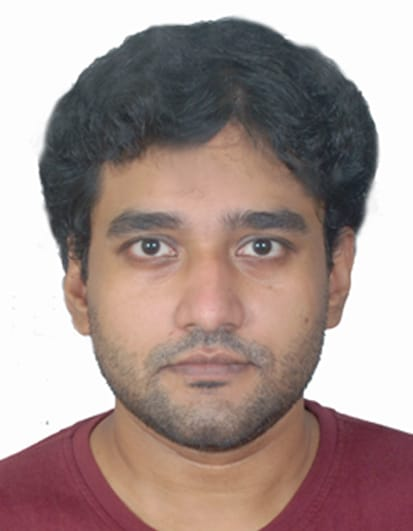
\includegraphics[width=0.13\textwidth]{images/shouvick2.jpg}~~~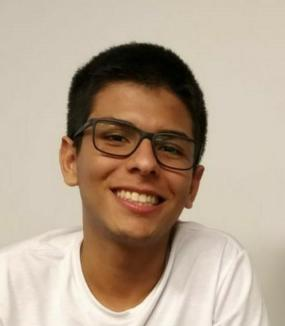
\includegraphics[width=0.15\textwidth]{images/denini.jpg}~~~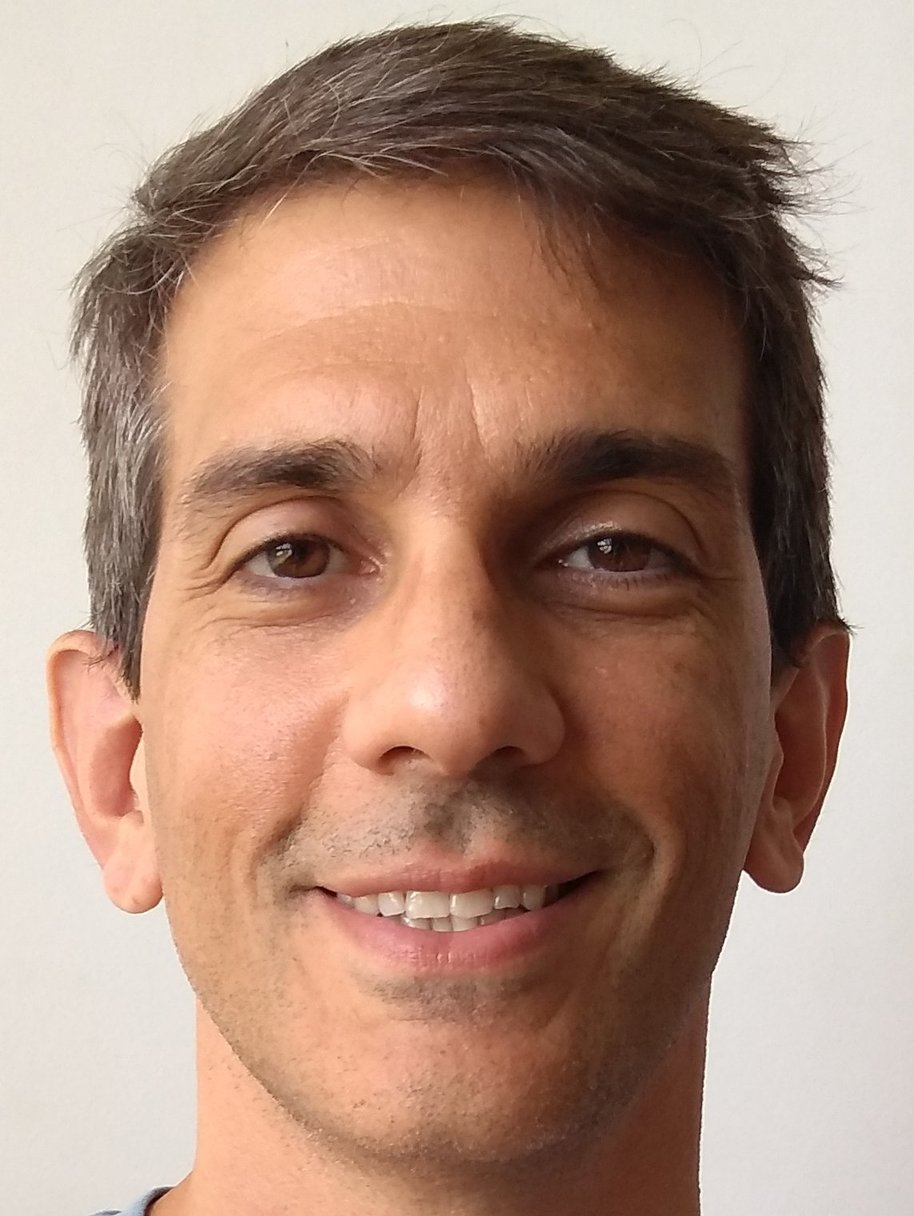
\includegraphics[width=0.13\textwidth]{images/marcelo.jpg}}
\date{ICSME 2021 (Virtual Event)\\{\scriptsize September 27 -- October 1}} % (optional, should be abbreviation of conference name)

%======================================================================================================

\begin{document}

\begingroup
\renewcommand{\disp}{}
\begin{frame}
	\titlepage
\end{frame}
\endgroup

\addtocounter{framenumber}{-1}

\begin{frame}{Context: software evolution and regression testing}
	
{\rsm Consider manipulating a function}:\\
$\{f(x)=2+x\}$ $\rightarrow$ $\{f'(x)=2*x\}$.\\
\vspace{0.3cm}
\pause
Inputs (test-cases): {\rsm 2}, {\rsm 4}\\
\textit{Expected} outputs: {\color{indiagreen}4}, {\color{indiagreen}6}\\\pause
\textit{Observed} outputs: {\color{indiagreen}4}, {\color{red}8}\\
\vspace{0.3cm}\pause
{\color{indiagreen}Functionality}: $f({\rsm 2})=f'({\rsm 2})=\color{indiagreen}4$ is still intact.\\
\vspace{0.3cm}\pause
\vspace{-4mm}
{\color{red} Failure} (functional discrepancy) revealed: $f({\rsm 4})\neq f'({\rsm 4})$.\\
\vspace{0.3cm}\pause
%{\color{blue}Root cause of failure}: The fault lies in our star *\\
%\vspace{0.3cm}\pause
{\textit{Relation with software testing}: RetestAll ({\color{red}\textit{expensive}!})}\\
Industrial example: RetestAll took seven weeks to complete!\onslide<6->\footnotemark\\\pause
\vfill
\textit{Sophisticated solutions}
\begin{itemize}
	\item{Regression test {\rsm selection} (RTS).}
	\item{Regression test {\rsm prioritization} (RTP).}
	\item{Test-suite {\rsm reduction} (TSR).}\pause
	\item{\textbf{\color{blue}\textit{Test-execution parallelization}} (or Test parallelization).}
\end{itemize}
\only<6->{\footnotetext[1]{\fontsize{4}{4}\selectfont\textbf{Source}: S. Elbaum et al., \textit{Prioritizing Test Cases for Regression Testing}, ISSTA 2000.}}
\end{frame}

\begin{frame}{Test parallelization levels}
	\centering
	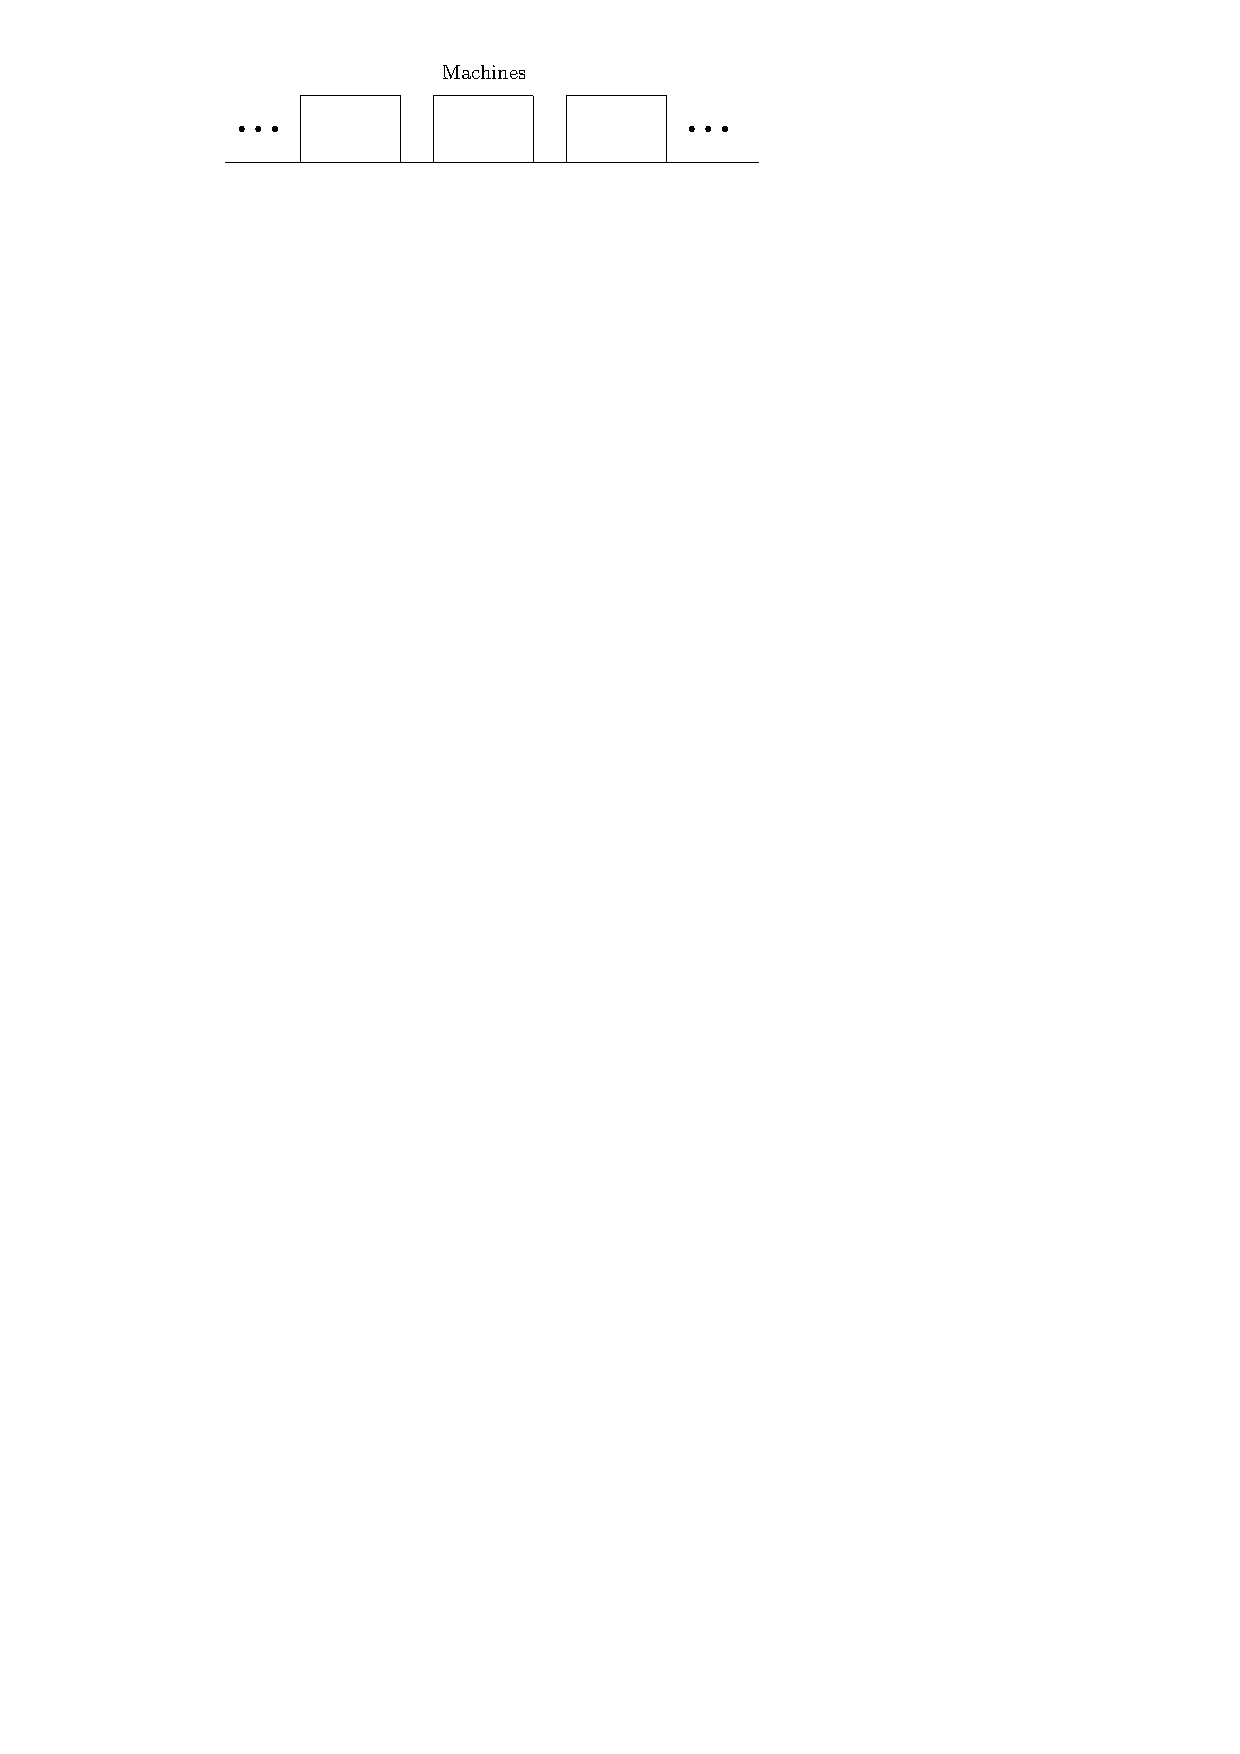
\includegraphics[width=\linewidth,page=1]{images/intro.pdf}
	\vfill
	{\color{white}In \tname{}, we have \textit{CPU} and \textit{thread} level parallelism.}
	\vfill
	{\fontsize{4}{4}\selectfont\textbf{Source}: J. Candido et al., \textit{Test suite parallelization in open-source projects: A study on its usage and impact}, ASE 2017.}
\end{frame}

\begin{frame}{Test parallelization levels}
	\centering
	\includegraphics[width=\linewidth,page=2]{images/intro.pdf}
\vfill
{\color{white}In \tname{}, we have \textit{CPU} and \textit{thread} level parallelism.}
\vfill
{\fontsize{4}{4}\selectfont\textbf{Source}: J. Candido et al., \textit{Test suite parallelization in open-source projects: A study on its usage and impact}, ASE 2017.}
\end{frame}

\begin{frame}{Test parallelization levels}
	\centering
	\includegraphics[width=\linewidth,page=3]{images/intro.pdf}
\vfill
In {\rsm \tname{}}, we have \textit{CPU} and \textit{thread} level parallelism.	
\vfill
\fontsize{4}{4}\selectfont\textbf{Source}: J. Candido et al., \textit{Test suite parallelization in open-source projects: A study on its usage and impact}, ASE 2017.
\end{frame}

\begin{frame}{Issues in test parallelization}
\begin{itemize}
	\item{Test flakiness.}
	\item{\underline{Test dependencies}.}
	\item{\underline{Data-races}.}
	\item{State pollution.}\pause
	\item{Test timeouts.}
	\item{Test monopolization}.\pause
	\item{Network connection.}
	\item{Disk + File I/O.}\pause
\end{itemize}
\vfill
{We \underline{\textit{may get}} a {\color{indiagreen}\textbf{good speedup}} but the {\color{red}\textbf{downside is reliability}}.}
\end{frame}

\begin{frame}{Some recent approaches towards test-parallelization}
\begin{center}
	\fontsize{7.5}{7.5}
	{	
		\selectfont
		\setlength{\tabcolsep}{0.9mm}
		\centering
		\begin{tabular}{l|l|r|l}
			\hline
			{\textbf{Work--venue}} & {\textbf{Languages used}} & {\textbf{Speedup}} & {\textbf{Machine type}}\\
			\hline
			{} & {} & {} & {}\\
			{{\rsm ElectricTest}--FSE 2015} & {\rsm Java} & {Avg. $16.00\times$} & {Amazon EC2}\\
			{} & {} & {} & {}\\
			\hline
			{} & {} & {} & {}\\
			%{{\rsm GPU execution}--ASE 2014} & {CUDA and {\rsm C (subset)}} & {Max. $27.00\times$} & {GPU}\\
			{{\rsm ParTeCL} (GPU)--ISSTA 2017} & {OpenCL and {\rsm C (subset)}} & {Avg. $16.00\times$} & {GPU}\\
			{} & {} & {} & {}\\
			\hline
			{} & {} & {} & {}\\
			{Candido et al.--ASE 2017} & {\rsm Java} & {Avg. $3.53\times$} & {8 cores @ 3.60 GHz}\\
			%{} & {Avg. $1.90\times$} & {80 cores @ 2.20 GHz}\\
			{({\rsm multi-core})} & {} & {Avg. $4.20\times$} & {80 cores @ 2.20 GHz}\\
			{} & {} & {} & {}\\
			\hline
			{} & {} & {} & {}\\
			{\mahtab--JSS 2019} & {C++, LLVM, and {\rsm C}} & {Avg. $5.17\times$} & {40 cores @ 2.40 GHz}\\
			%{} & {Avg. $1.90\times$} & {80 cores @ 2.20 GHz}\\
			{({\rsm multi-core})} & {} & {G.M. $4.72\times$} & {40 cores @ 2.40 GHz}\\
			{} & {} & {} & {}\\
			\hline
		\end{tabular}
	}	
\end{center}
\centering
{\fontsize{9}{9}\selectfont We \underline{\textit{may get}} a {\color{indiagreen}\textbf{good speedup}}.}
\end{frame}

\begin{frame}{Our solution: \tname{}}
\begin{itemize}
\item{\textbf{\tname}~({\rsm \textbf{PArallel-Sequential Test Execution}}), an approach to \textit{\rsm \underline{automate}} parallel execution of tests.}\pause
\item{\tname\ builds on the observation that {\rsm \textit{\underline{broken test dependencies}}} that are manifested in parallel runs {\rsm \textit{\underline{involve test cases from the same test class}}}.}\pause
\item{\tname\ leverages that observation to \textit{\rsm \underline{reinstate those dependencies by running}} the tests from the same class in the same order.}\pause
\item{\tname\ is organized as a pipeline of \textit{\underline{three stages}}.}
\end{itemize} 
\end{frame}

\begin{frame}{\tname{}: the three-staged pipeline of test execution}
	\centering 
	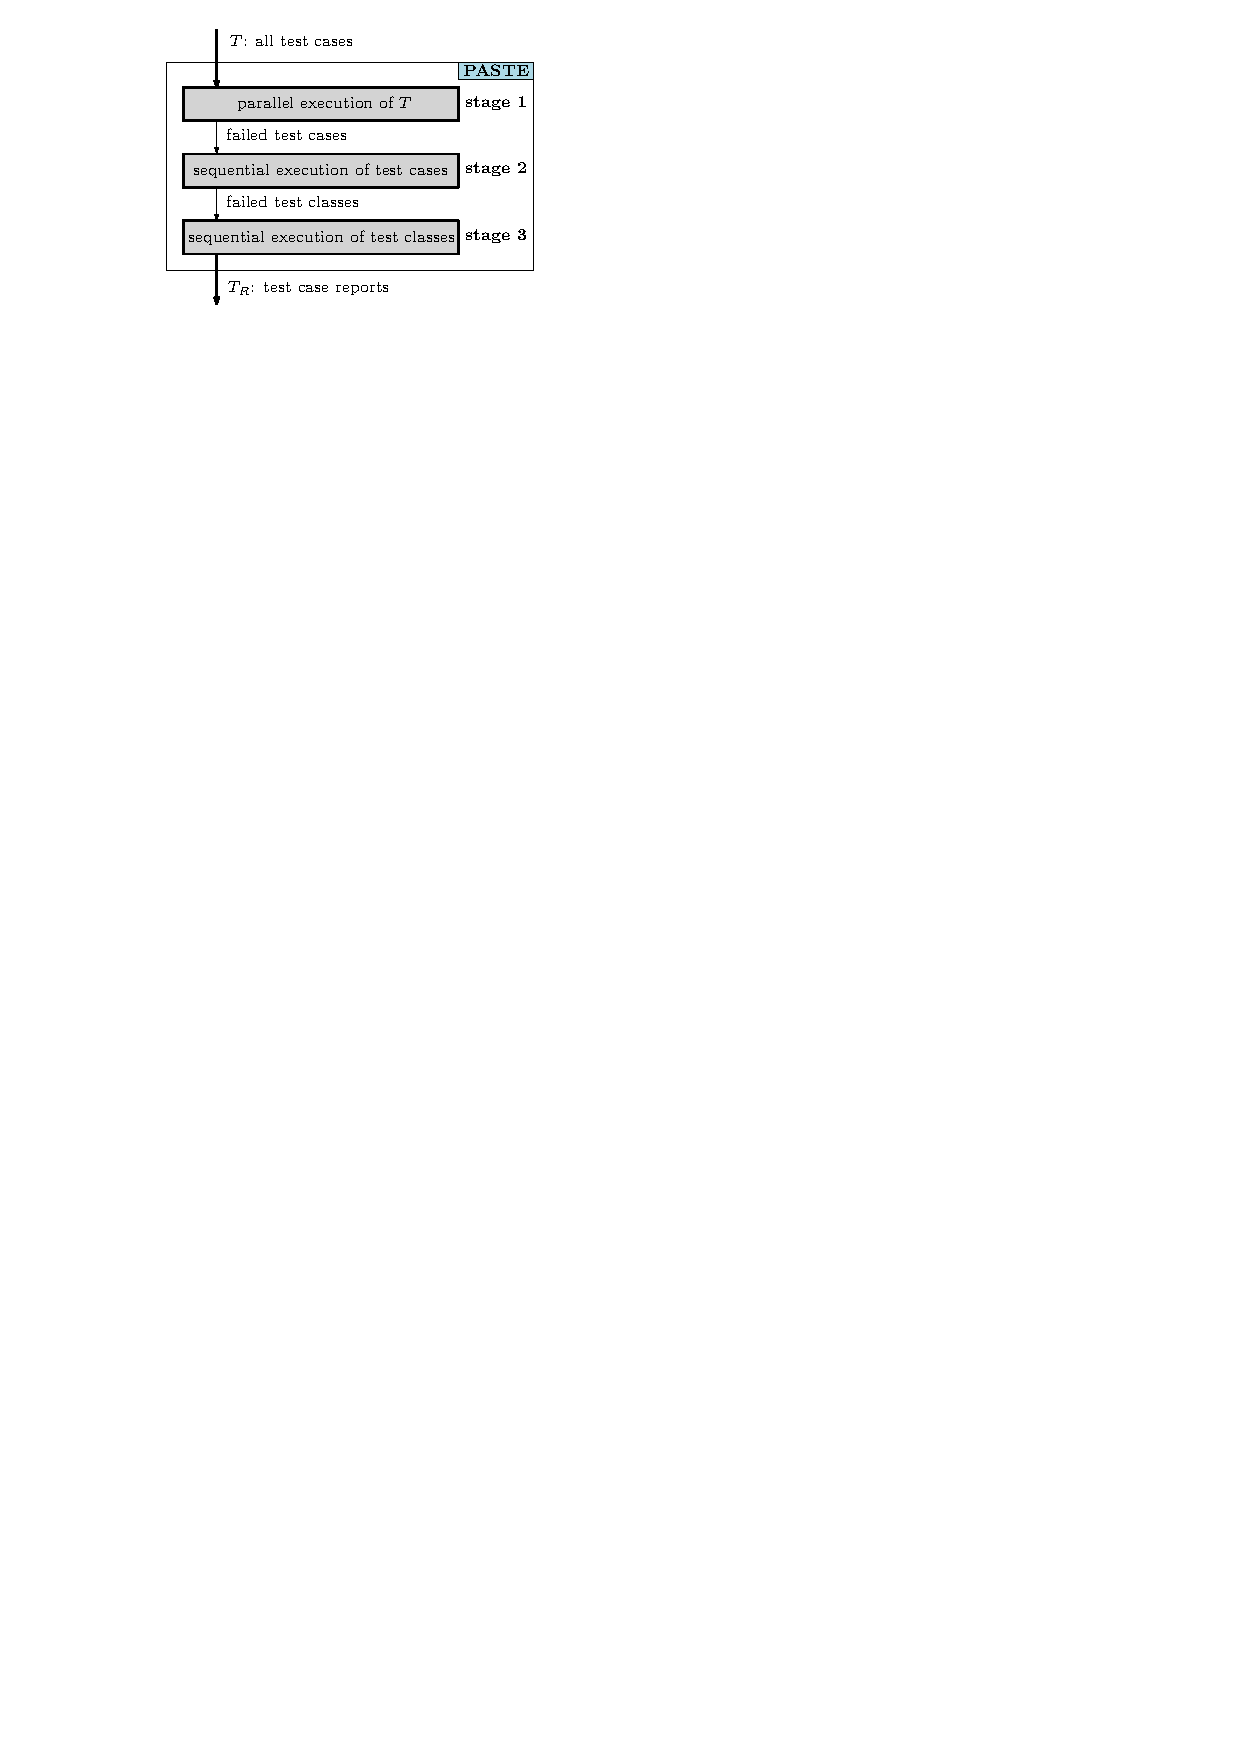
\includegraphics[width=0.8\linewidth]{images/soundy.pdf}
\end{frame}

%\begin{frame}[fragile]{The setting: software evolution and regression testing}
%\vspace{-0.15cm}
%\begin{center}
%\begin{figure}
%\begin{minipage}{1.0\textwidth}
%\centering
%\begin{tabular}{r@{\hskip 0.08\textwidth}l}
%{\begin{lstlisting}
%// source_v0.c
%#include<stdio.h>
%...
%int main()
%{
%	int n;
%	scanf("%d", &n);
%	if(n % 2 == 0)
%	{
%		...
%	}
%	else
%	...
%}
%\end{lstlisting}}
%&
%{\begin{lstlisting}	
%// source_v1.c	
%#include<stdio.h>
%...
%int main()
%{
%	int n;
%	scanf("%d", &n);
%	if(n % 2 == 0)
%	{
%		...
%		|{\color{indiagreen} \textbf{n = n - 32000;}}| //change|\label{line:v1}|
%	}
%	else
%	...
%}
%\end{lstlisting}}%
%\end{tabular}
%\vspace{-0.8cm}
%\caption{\footnotesize Original source code (\textit{\rsm source\_v0.c}) and its new version (\textit{\rsm source\_v1.c}).}
%\label{fig:source2}
%\end{minipage}
%\end{figure}
%\end{center}
%\begin{center}
%\vspace{-0.5cm}\pause
%\footnotesize
%{\rsm $\Sigma$}: $\{t_1,t_2,t_3,...,t_{10}\}$ (original test-suite)\\\pause
%{\rsm $\{t_1,...,t_{10}\}$}: (contains randomly generated integer in $[0..99]$)\\\pause
%{\rsm $\{0,4,16,50,2\}$}: (integers present in $\{t_1,t_3,t_5,t_7,t_9\}$)\\\pause
%{\rsm All other test-cases} $\in{\Sigma}$ contain odd numbers in $[0..99]$
%\end{center}
%\vspace{-0.3cm}
%\begin{center}
%\fontsize{7.75}{7.75}{
%	\begin{center}\pause
%		\fontsize{7.75}{7.75}{What are we testing for?\selectfont}
%		\begin{itemize}
%			\item[]{\textbf{\color{red}\textit{Failure}}: An {\rsm event} that occurs when {\rsm current} service {\rsm deviates} from {\rsm expected} service.}\pause
%			%\item[]{\textbf{\color{red}Error}: A system {\rsm state} or {\rsm configuration} that might {\rsm cause} a {\rsm failure}.}\pause
%			%\item[]{\textbf{\color{red}Fault}: The {\rsm root cause} which gives rise to an {\rsm error}.}\pause
%		\end{itemize}
%	\end{center}
%	\selectfont}
%\end{center}
%\begin{center}
%\vspace{-1mm}
%\begin{itemize}
%	\centering
%	\item[]{\scriptsize\color{blue}Testing may consume over $80\%$ \textit{end-to-end}, and $50\%$ maintenance cost.}\onslide<7->\footnotemark
%\end{itemize}
%\end{center}
%\only<7->{\footnotetext[2]{\fontsize{4.5}{4.5}\selectfont\textbf{Source}: A. Bertolino, \textit{Software Testing Research: Achievements, Challenges, Dreams}, FOSE 2007.}}
%\end{frame}
%
%\begin{frame}[t]{Motivation: parallelization of regression testing}
%	\vspace{-0.3cm}
%	\begin{center}
%		\begin{itemize}
%			\item{{Three phases} of regression testing}
%			\begin{itemize}
%				\item{{\rsm Offline}: Code {\rsm instrumentation} and {\rsm test-coverage} map generation \{{\color{gray} test-cases} $\rightarrow$ {\color{red} code-elements}\}.}\pause
%				\item{{\rsm Online}: Identify {\rsm changed elements}, use reverse mapping \{{\color{red} code-elements} $\rightarrow$ {\color{gray} test-cases}\} to {\rsm select regression tests}.}\pause
%				\item{{\rsm Execution}: Execute {\rsm selected} tests.}\pause
%			\end{itemize}
%		\end{itemize}
%		\begin{figure}[h]
%			\begin{center}
%				\includegraphics[scale=0.7,page=2]{images/dep.pdf}
%			\end{center}
%		\end{figure}
%		\vfill\pause
%		{\footnotesize
%			{\color{red}None of the prior works targeted phase-wise parallelization!}\pause\\
%			{\color{blue}We propose parallelization windows to achieve this.}}\pause
%		\\
%		{\fontsize{7}{7}\selectfont{\rsm Assumption}: All test-cases are \textit{independent}\onslide<7->\footnotemark and can be executed in \textit{parallel}.}
%		\only<7->{\footnotetext[3]{\fontsize{4}{4}\selectfont\textbf{Source}: M. J. Harrold et al., \textit{Regression Test Selection for Java Software}, OOPSLA 2001.}}
%	\end{center}
%\end{frame}
%
%\begingroup
%\renewcommand{\disp}{}
%\begin{frame}
%	\begin{center}
%		Parallelization windows
%	\end{center}
%\end{frame}
%\endgroup
%
%\addtocounter{framenumber}{-1}
%
%\begin{frame}{Illustration of parallelization windows}
%	\begin{center}
%		\begin{figure}
%			\includegraphics[scale=1.2,page=4]{images/Mahtab.pdf}
%			\caption{\footnotesize {\rsm Executing selected} tests: sequential versus {\rsm parallel windows} (shaded in gray).}
%		\end{figure}
%	\end{center}
%\end{frame}
%
%\begin{frame}{Thesis contribution placement diagram}
%\begin{center}
%	\begin{figure}[h]
%		\begin{center}
%			\includegraphics[width=0.9\linewidth]{images/flow.pdf}	
%		\end{center}
%	\end{figure}
%	\begin{itemize}
%		\item{{\color{darkred}\mahtab}: Phase-wise acceleration of regression testing.}
%		\item{{\color{blue}\hansie}: Consensus test-case prioritization.}
%		\item{{\color{blue}\colosseum}: Delta-displacement based prioritization.}
%	\end{itemize}
%\end{center}
%\end{frame}
%
%\begin{frame}
%	\begin{center}
%		\begin{itemize}
%			\item{\textbf{{\rsm Contribution \#1 (JSS 2019 journal paper)}\\\mahtab: Phase-wise acceleration of regression testing}}
%			\item{\color{lightgray}Contribution \#2 (JSS 2021 journal paper)\\\hansie: Consensus test-case prioritization}
%			\item{\color{lightgray}Contribution \#3 (Journal submission)\\\colosseum: Delta-displacement based prioritization}
%		\end{itemize}
%	\end{center}
%\end{frame}
%
%\begin{frame}{Parallelization in the \textit{offline} phase}
%\begin{center}
%	\begin{figure}[h]
%		\begin{center}
%			\includegraphics[scale=0.55,page=1]{images/dep2.pdf}
%		\end{center}
%	\end{figure}
%\end{center}
%\end{frame}
%
%\begin{frame}{Parallelization in the \textit{online} phase}
%	\begin{center}
%		\begin{figure}[h]
%			\begin{center}
%				\includegraphics[scale=0.55,page=2]{images/dep2.pdf}
%			\end{center}
%		\end{figure}
%	\end{center}
%\end{frame}
%
%\begin{frame}{Parallelization in the \textit{execution} phase}
%	\begin{center}
%		\begin{figure}[h]
%			\begin{center}
%				\includegraphics[scale=0.55,page=3]{images/dep2.pdf}
%			\end{center}
%		\end{figure}
%	\end{center}
%\end{frame}
%
%\begin{frame}{\textit{End-to-end} parallelization}
%	\begin{center}
%		\begin{figure}[h]
%			\begin{center}
%				\includegraphics[scale=0.55,page=5]{images/dep2.pdf}
%			\end{center}
%		\end{figure}
%	\end{center}
%\end{frame}
%
%\begin{frame}
%	\begin{center}
%		\begin{itemize}
%			\item[]{\color{lightgray}Contribution \#1 (JSS 2019 journal paper)\\\mahtab: Phase-wise acceleration of regression testing}
%			\item{\textbf{{\rsm Contribution \#2 (JSS 2021 journal paper)}\\\hansie: Consensus test-case prioritization}}
%			\item[]{\color{lightgray}Contribution \#3 (Journal submission)\\\colosseum: Delta-displacement based prioritization}
%		\end{itemize}
%	\end{center}
%\end{frame}
%
%\begin{frame}{Prioritized test-execution: traditional vs. consensus}
%
%{{\rsm \textit{Prioritization}}: Execute those test-cases \textit{\rsm earlier} which are capable of {\rsm revealing failures.}\\\pause}
%\vfill
%{\color{blue} A single heuristic may not perform optimally in all scenarios!\pause\\A \textit{consensus} may be better.\\}
%\vfill
%$\sigma$: $\{t_1,t_3,t_5,t_7,t_9\}$ (regression test-suite)\\
%$p_1$: $<$\sm{$t_3$}, $t_1$, \sm{$t_5$}, $t_9$, \sm{$t_7$}$>$ (prioritization due to heuristic \#1)\\\pause
%$p_2$: $<$\sm{$t_5$}, $t_9$, \sm{$t_3$}, \sm{$t_{7}$}, $t_1$$>$ (prioritization due to heuristic \#2)\\\pause
%$p_3$: $<$\sm{$t_{7}$}, $t_1$, \sm{$t_5$}, \sm{$t_3$}, $t_9$$>$ (prioritization due to heuristic \#3)\\\pause
%\fbox{{\rsm $p^*$}: $<$\sm{$t_5$}, \sm{$t_3$}, $t_1$, \sm{$t_7$}, $t_9$$>$ ({\rsm consensus prioritization})}\onslide<6->\footnotemark\\\pause
%$p_{opt}$: $<$\sm{$t_3$}, \sm{$t_5$}, \sm{$t_7$}, $t_1$, $t_9$$>$ (\textit{optimal} prioritization)\\
%\vfill
%\onslide<3->
%%\begin{center}
%{\footnotesize
%For our example code revision: \textit{failed} test-cases are highlighted in {\color{red}red}. \pause{\rsm Note that we do not know apriori which test-case will fail!}} \pause
%\onslide<9->{\footnotesize A {\rsm dense} distribution of {\rsm failed} test-cases observed {\rsm near the beginning} of the timeline is desirable}\onslide<9->\footnotemark
%%\end{center}
%\onslide<6->
%\only<6->{\footnotetext[4]{\fontsize{4.5}{4.5}\selectfont\textbf{Source}: W. Press, \textit{C++ Program for Kemeny-Young Preference Aggregation}, [Online] 2012.}}
%\only<9->{\footnotetext[5]{\fontsize{4.5}{4.5}\selectfont\textbf{Source}: W. Torres, \textit{An Empirical Study on the Spreading of Fault Revealing Test Cases in Prioritized Suites}, COMPSAC 2019.}}
%\end{frame}
%
%\begin{frame}[t]{Major contributions of \hansie}
%\begin{itemize}
%	\item{We perform a study on \textit{\rsm hybrid} (on-the-fly), and \textit{\rsm consensus} (post-individual) regression test {\rsm \textit{prioritization}} techniques.}\pause
%	%\item{We introduce a \textit{visual interpretation} of comparing effectiveness of multiple prioritization approaches, in terms of: (i) \textit{failure positions}, and (ii) \textit{permutation shuffles}.}
%	\item{We introduce {\rsm \textit{\hansie} \textit{distance}} between two prioritizations (with and without ties) to measure the \textit{\rsm quality} of the {\rsm \textit{final consensus}} prioritization.}\pause
%	\item{We introduce {\rsm \textit{EPL$_\omega$}}, a \textit{cost-cognizant metric} for quantifying \textit{\rsm effectiveness} of {\rsm \textit{prioritization-parallelization}}, when execution is driven by \textit{\rsm size-varying} test-parallelization windows of \textit{\rsm unequal load} distribution.}
%\end{itemize}
%\end{frame}
%
%\begin{frame}
%	\begin{center}
%		\begin{itemize}
%			\item{\color{lightgray}Contribution \#1 (JSS 2019 journal paper)\\\mahtab: Phase-wise acceleration of regression testing}
%			\item{\color{lightgray}Contribution \#2 (JSS 2021 journal paper)\\\hansie: Consensus test-case prioritization}
%			\item{\textbf{{\rsm Contribution \#3 (Journal submission)}\\\colosseum: Delta-displacement based prioritization}}
%		\end{itemize}
%	\end{center}
%\end{frame}
%
%\begin{frame}{Tri-partition of test-coverage path and displacements}
%\vspace{-0.4cm}
%\begin{figure}[h]
%\begin{center}
%	\includegraphics[width=\columnwidth,page=3]{images/colosseum.pdf}
%\end{center}
%\vspace{-0.4cm}
%\onslide<3->{
%{\fontsize{10.25}{10.25}\selectfont
%	\begin{eqnarray*}
%		d_{val}(t_i)=\left\{\frac{(a+1)\times(b+1)\times(c+1)}{max\{d_{val}\}}\right\}\label{eqn:dval}
%\end{eqnarray*}}}
%\end{figure}
%\vspace{-0.5cm}\pause
%\begin{itemize}
%	\item{\textit{\rsm Delta-displacement triple}: tri-partition of a {\rsm loop-free in-order} basic-block coverage of a test-case execution path in the older version of the code. {\rsm $(a,b,c)$} is the {delta displacement triple} for test-case $t_i$.}\pause
%	\item{A {\rsm shorter overall displacement} has a low chance of getting affected by the {\rsm computational masking} \pause which acts as a strong inhibitor of {\rsm change propagation} to the output\pause, rendering the {\rsm test-case coincidentally correct}.}
%\end{itemize}
%\end{frame}
%
%\begin{frame}[t]{Major contributions of \colosseum}
%\begin{itemize}
%	\item{We propose the {\rsm \textit{first}} prioritization strategy, \colosseum, that takes into account the {\rsm \textit{position}} of {\rsm \textit{changed}} code elements {\rsm \textit{along the execution path}} of regression test-cases.}\pause
%	\item{We introduce a heuristic that {\rsm \textit{approximates}} the {\rsm \textit{immunity}} of a test-case to {\rsm \textit{change-masking}} (coincidental correctness) by code-change {\rsm \textit{displacements}}.}\pause
%	\item{We introduce the notion of {\rsm \textit{PriOritized Window Execution Request}} (\textit{\rsm POWER}) tree for \textit{parallel test-execution}.}
%\end{itemize}
%\end{frame}
%
%\begingroup
%\renewcommand{\disp}{}
%\begin{frame}
%	\begin{center}
%		Experimental Results
%	\end{center}
%\end{frame}
%\endgroup
%
%\addtocounter{framenumber}{-1}
%
%\begin{frame}[t]{Benchmarks}
%	\begin{center}
%			\textit{Benchmarks}: {Obtained from SIR\onslide<1->\footnotemark repository, and GitHub\onslide<1->\footnotemark }.
%			\begin{itemize}
%				\item{20 open-source projects.}
%				\item{280 versions.}
%				\item{69,305 test-cases.}
%				\item{80,338 delta blocks.}
%				\item{694,512 lines of source code.}
%			\end{itemize}
%		\only<1->{\footnotetext[6]{\fontsize{6}{6}\selectfont\textbf{Source}: https://sir.unl.edu/portal/index.php (12 out of 15 benchmarks).}}
%		\only<1->{\footnotetext[7]{\fontsize{6}{6}\selectfont\textbf{Source}: https://github.com (8 active projects).}}
%	\end{center}
%\end{frame}
%
%\begin{frame}{Evaluation}
%\begin{center}
%\mahtab: phase-wise acceleration
%\begin{tcolorbox}
%{\fontsize{10.25}{10.25}\selectfont
%End-to-end speedup (against sequential RTS) for SIR and GitHub: \textbf{\color{blue} $\mathbf{4.72\times}$ with $\mathbf{16}$ threads}, and {\textbf{\color{blue} $\mathbf{3.04\times}$ with $\mathbf{32}$ threads.}
%}}
%\end{tcolorbox}
%\pause{
%\hansie: consensus prioritization
%\begin{tcolorbox}
%{\fontsize{10.25}{10.25}\selectfont
%\textit{13 individual prioritizations, 6 consensus operators. A consensus operator aggregates all 13 rankings.} 
%(consensus prioritization effectiveness ordering $\succ$):\\{\color{blue}\textit{\textbf{HM} $\succ$ \textit{\textbf{GM}} $\succ$ \textit{\textbf{AM}} $\succ$ \textit{\textbf{Borda}} $\succ$ \textit{\textbf{med.}} $\succ$ \textit{\textbf{Kem.}}}}
%}
%\end{tcolorbox}
%}
%\pause{
%\colosseum: delta-displacement based prioritization
%\begin{tcolorbox}
%{\fontsize{10.25}{10.25}\selectfont
%Overall success: {\color{blue}$\mathbf{84.61\%}$} (\textit{best performing strategy in terms of 11 out of 13 prioritization effectiveness metrics}).
%}
%\end{tcolorbox}}
%\end{center}
%\end{frame}

\begin{frame}{Conclusions}
\begin{itemize}
	\item{\footnotesize We discussed {\rsm \tname{}}, a lightweight approach to {\rsm \underline{parallelize execution}} of test suites through the {\rsm \underline{sequential re-execution} of \textit{test cases}} (\textit{to avoid data races}) and the {\rsm \underline{sequential re-execution} of \textit{test classes}} (\textit{to avoid broken test dependencies}).}
\end{itemize}
\begin{center}
\begin{figure}[!htb]
\centering
\begin{minipage}{0.475\textwidth}
	\centering
	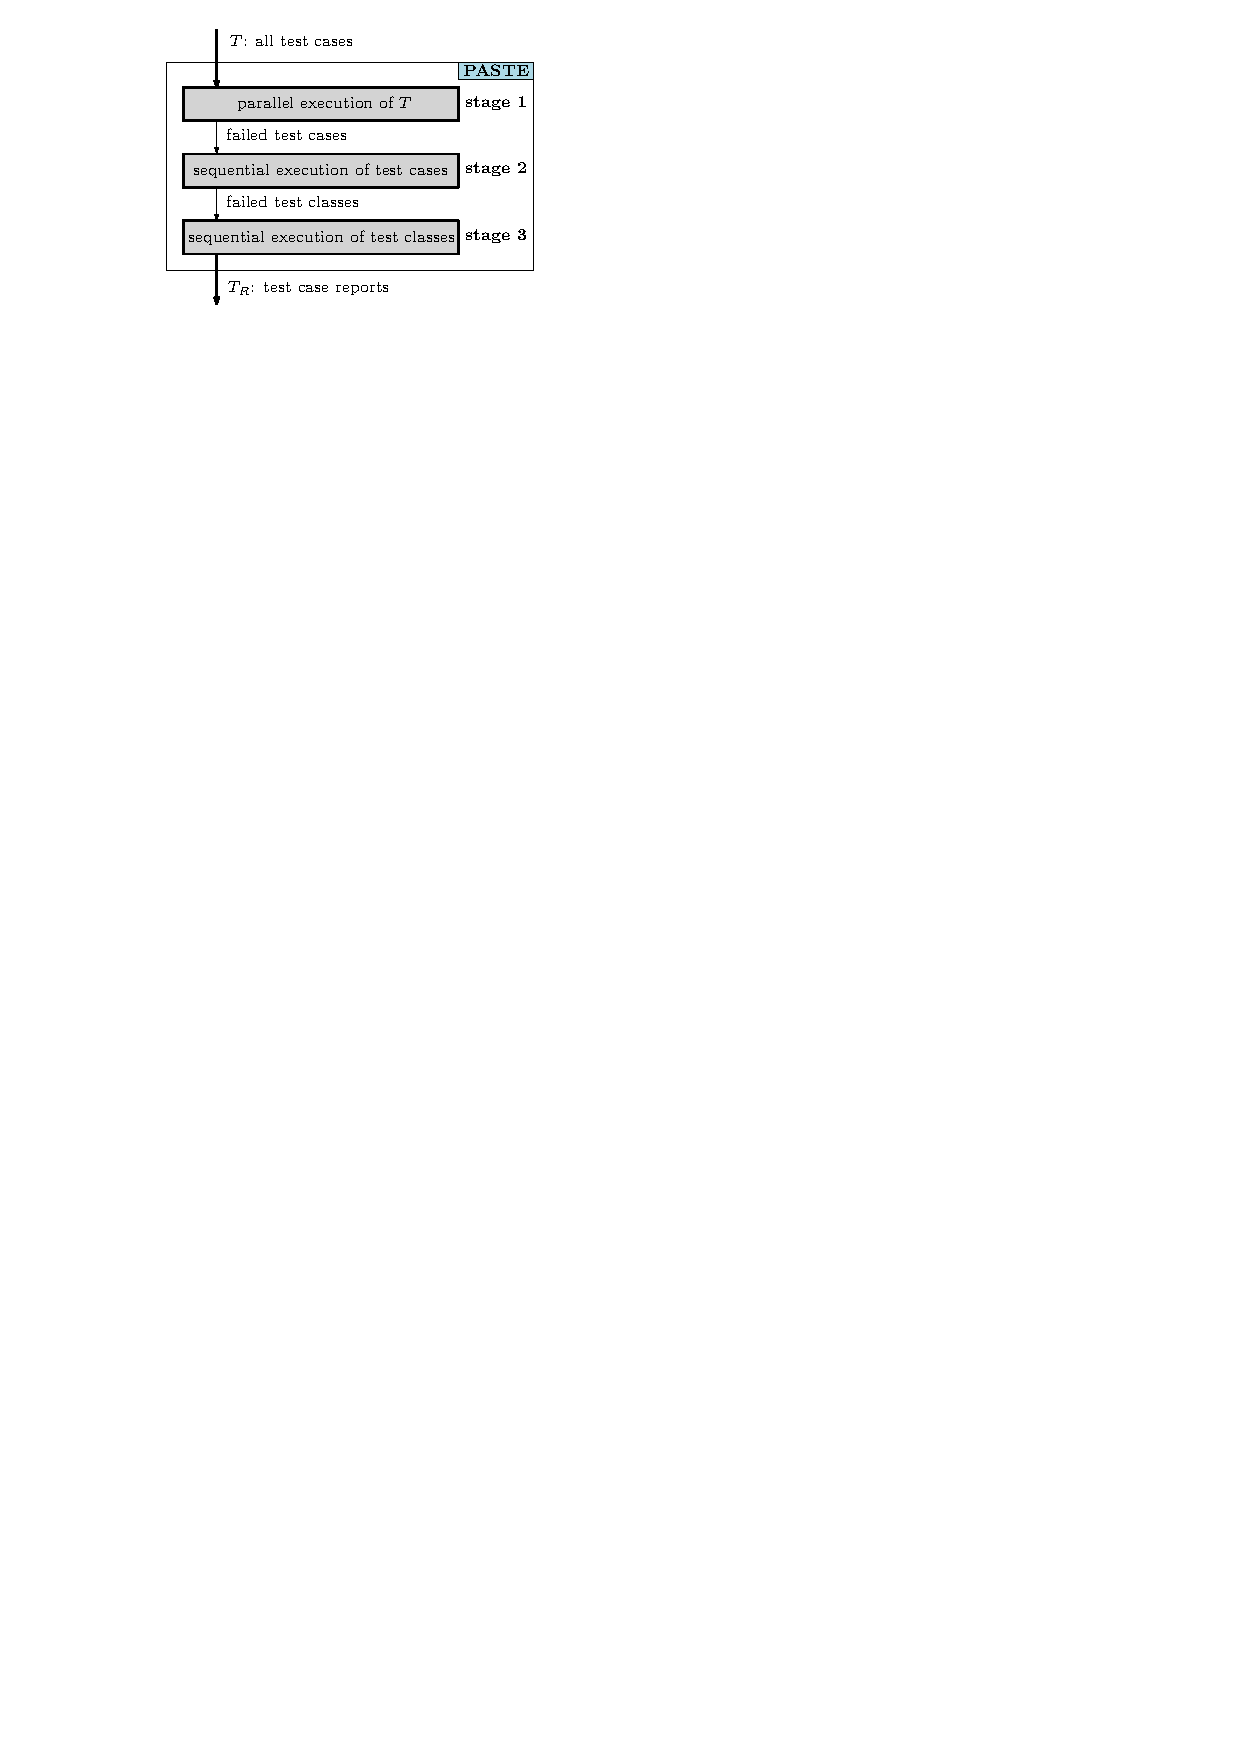
\includegraphics[width=\linewidth]{images/soundy.pdf}	
\end{minipage}%
\pause
\begin{minipage}{0.5\textwidth}
	\centering
	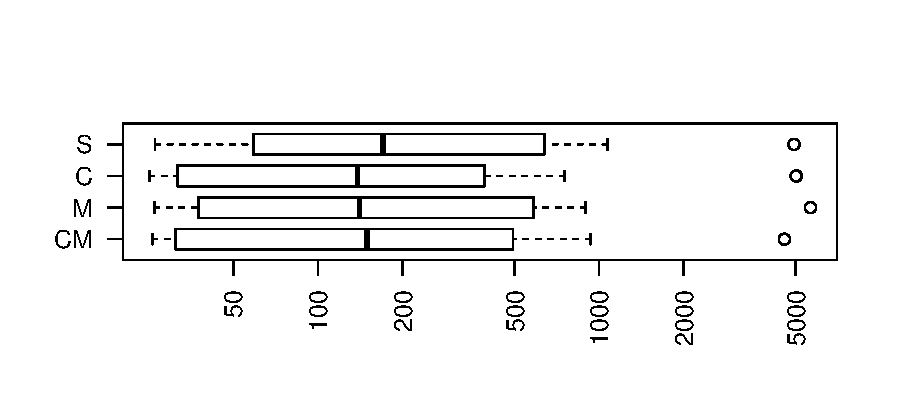
\includegraphics[width=1.175\linewidth]{images/time.pdf}\vspace{-1cm}
	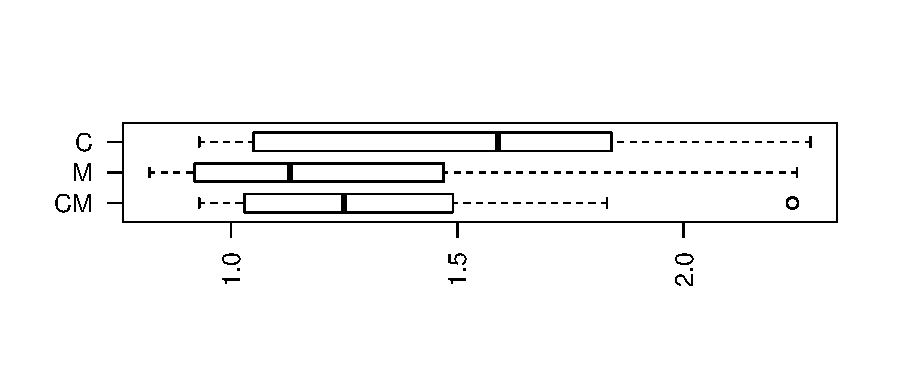
\includegraphics[width=1.175\linewidth]{images/speedup.pdf}	
\end{minipage}
\end{figure}	
\vfill
\vfill
\pause
\begin{Large}
	Thank You
\end{Large}
\vfill
\begin{footnotesize}
	Artifacts: \url{https://github.com/STAR-RG/paste}\\
	E-mail: \href{mailto:shouvick.mondal.cemk@gmail.com}{\texttt{shouvick.mondal.cemk@gmail.com}}
\end{footnotesize}
\end{center}
\end{frame}

%======================================================================================================

\renewcommand{\disp}{}

\appendix
\backupbegin

\begin{frame}
	\begin{center}
		{\huge Backup Slides}
	\end{center}
\end{frame}

%\begingroup
%\renewcommand{\disp}{}
%\begin{frame}
%	\begin{center}
%		Measuring effectiveness of prioritization-parallelization
%	\end{center}
%\end{frame}
%\endgroup

%\addtocounter{framenumber}{-1}

%\begin{frame}{Area under the curve: failure detection effectiveness}
%	\begin{figure}[h]
%		\begin{center}
%			\fbox{\includegraphics[scale=0.55]{images/prio_vis.pdf}}
%		\end{center}
%		\vfill
%		%\caption{\centering\footnotesize {\rsm Cumulative observance of test failures} due to individual ($p_1, p_2, p_3$), consensus ($p^*$), and optimal ($p_{opt}$) prioritizations. {\rsm $y$-axis label indicates cumulative failures up to each $x$}, and assumes no ordering among $p_i$s.}
%		%\label{fig:demo_prio_vis}
%	\end{figure}
%	\begin{itemize}
%		\footnotesize
%		\item{{\rsm Cumulative observance of test failures} due to individual ($p_1, p_2, p_3$), consensus ($p^*$), and optimal ($p_{opt}$) prioritizations.}\pause
%		\item{{\rsm $y$-axis label indicates cumulative failures up to each $x$}, and assumes no ordering among $p_i$s.}\pause
%		\item{The {\color{indiagreen} greater the area} under the curve, {\color{indiagreen}the better} is the prioritization effectiveness in terms of {\color{red}failure observation rate}.}
%	\end{itemize}
%\end{frame}
%
%\begin{frame}{Measuring effectiveness of prioritization-parallelization}
%	\begin{center}
%		\begin{itemize}
%			\item{Average Percentage {Faults Detected} ({\rsm APFD}).}
%			\begin{itemize}
%				\item[]{Rewards {\rsm early fault detection}.}
%				\item[]{Assumes all test-cases have {\rsm same execution cost}.}
%			\end{itemize}\pause
%			\item{Cost-cognizant APFD ({\rsm APFD$_c$}).}
%			\begin{itemize}
%				\item[]{Rewards {\rsm early fault detection}.}
%				\item[]{Considers test-cases with {\rsm different execution costs}.}
%			\end{itemize}\pause
%			\item{Effectiveness of {Change Coverage} ({\rsm ECC}).}\begin{itemize}
%				\item[]{Rewards {\rsm early change coverage}.}
%			\end{itemize}\pause
%			\item{EPSilon ({\rsm EPS}) and EPSilon$_\omega$ ({\rsm EPS$_\omega$}): \mahtab's metric based on {similarity with optimal prioritization}.}\begin{itemize}
%				\item[]{Rewards {\rsm early failure observation}.}
%			\end{itemize}
%			%\pause
%			%			\item{EPSilon-Latency ({\rsm EPL$_\omega$}): \hansie's metric for {\rsm end-to-end execution timeline latency} due to parallelization windows.}\pause
%			%			\begin{equation*}
%			%				\textnormal{\textit{EPL$_\omega$}}=1-\left\lbrack{\frac{c_1.\log_2(n+1)+c_2.\log_2n+...+c_n.\log_22}{c_{max}.\{\log_2{(n+1)}+\log_2n+...+\log_22\}}}\right\rbrack\label{eqn:one}
%			%			\end{equation*}
%		\end{itemize}
%		\vfill\pause
%		{\footnotesize\color{blue} These metrics get quantified (normalized within $[{\color{red}0},{\color{indiagreen}\textbf{1}}]$)\\\textit{only after} test-execution respecting priority.}
%	\end{center}
%\end{frame}

\backupend

\end{document}